% Shared preamble for the MIRAGE report and supplementary document
\documentclass[10pt,a4paper,twocolumn]{article}
\usepackage[a4paper,top=1.6cm,bottom=1.6cm,left=1.5cm,right=1.5cm,columnsep=0.7cm]{geometry}
\usepackage[T1]{fontenc}
\usepackage[utf8]{inputenc}
\usepackage{times}
\usepackage{microtype}
\usepackage{graphicx}
\usepackage{booktabs}
\usepackage{array}
\usepackage{tabularx}
\usepackage{longtable}
\usepackage{caption}
\usepackage{subcaption}
\usepackage{amsmath}
\usepackage{siunitx}
\usepackage{xcolor}
\usepackage{enumitem}
\usepackage{titlesec}
\usepackage{hyperref}
\usepackage{xurl}
\usepackage{float}
\usepackage{setspace}

\definecolor{mirageblue}{HTML}{1F4E79}
\definecolor{mirageink}{HTML}{222222}
\hypersetup{colorlinks=true,linkcolor=mirageblue,citecolor=mirageblue,urlcolor=mirageblue,pdftitle={MIRAGE: Measuring the Impact and Reality of Rainwater Harvesting Mandates}}

\titleformat{\section}{\normalfont\fontsize{10.5}{12}\bfseries\color{mirageblue}}{\thesection}{0.5em}{}
\titleformat{\subsection}{\normalfont\fontsize{10}{12}\bfseries}{\thesubsection}{0.5em}{}
\titlespacing*{\section}{0pt}{6pt plus 2pt minus 1pt}{3pt}
\titlespacing*{\subsection}{0pt}{4pt plus 1pt minus 1pt}{2pt}
\captionsetup{font=small,labelfont=bf,skip=3pt}
\setlist{nosep,leftmargin=1.2em}
\setlength{\parskip}{2pt}
\setlength{\parindent}{0pt}
\sisetup{group-separator={,},group-minimum-digits=4}
\renewcommand{\arraystretch}{1.12}
\newcommand{\inr}{Rs}

\usepackage{dblfloatfix}
\geometry{top=1.3cm,bottom=1.3cm,left=1.3cm,right=1.3cm,columnsep=0.6cm}
\renewcommand{\normalsize}{\fontsize{8.7}{10.1}\selectfont}
\normalsize
\renewcommand{\topfraction}{0.95}\renewcommand{\bottomfraction}{0.6}\renewcommand{\textfraction}{0.03}\renewcommand{\floatpagefraction}{0.9}\renewcommand{\dbltopfraction}{0.95}\renewcommand{\dblfloatpagefraction}{0.95}\setcounter{dbltopnumber}{4}\setcounter{topnumber}{4}\setcounter{totalnumber}{6}\setlength{\floatsep}{5pt}\setlength{\textfloatsep}{7pt}\setlength{\dbltextfloatsep}{7pt}\setlength{\dblfloatsep}{5pt}
\begin{document}

\twocolumn[{%
\begin{center}
{\LARGE\bfseries\color{mirageblue} MIRAGE: Measuring the Impact and Reality of Rainwater Harvesting Mandates}\\[3pt]
{\large A meta-analysis of rooftop rainwater harvesting performance in Indian cities}\\[5pt]
{\normalsize Vedant Abhangrao (23B2262) \,|\, Nilay Shahapure (23B2206) \,|\, Arjun Jhunjhunwala (23B1245) \,|\, Yash Krishnani (23B1240)}\\[2pt]
{\small CM617 Sustainability Principles and Practices, IIT Bombay. Course project, Pathway 1 (Sustainability Research), Water sector. October 2026.}
\end{center}
\vspace{2pt}
\begin{minipage}{\textwidth}
\small
\textbf{Abstract.} Indian cities have made rooftop rainwater harvesting (RWH) compulsory for over twenty years, but there is no consolidated quantitative evidence on whether installed systems deliver what their designs promise. We screened 89 published site records, 43 cost records, 46 surveys and audits, and 24 mandate instruments, and compared reported harvested or recharged volumes with theoretical potential (catchment area $\times$ rainfall $\times$ runoff coefficient) for 35 observations at 31 sites. Sites where the source names a flow meter, measuring device or tank record delivered a median 28\% of potential (n\,=\,7, 5 sites), while volumes reported by agencies without a stated measurement method had a median of 99\%, with 5 of 9 at or above 99\%: design estimates, not measurements (Mann-Whitney $p=0.023$; $p=0.001$ if one borderline case is regraded). Thirteen survey estimates put a median 40\% of installed systems functional. Levelised cost of harvested water has a median of Rs~21 per kL at design yield (2024 rupees) and about Rs~42 at observed yield; the median is below tanker prices at either yield; the most recent systems are not. Chaining the Chennai installation rate (60\%), functional share (77\% of installed) and observed yield ratio, the mandate delivers roughly 13\% of the water it targets. No agency measures what the mandate delivers. The few measurements fall well short of design. The reported failures point to maintenance and enforcement, not cost.
\end{minipage}
\vspace{6pt}
}]

\section{Introduction}
Chennai made RWH compulsory for every building in 2003; Bengaluru, Delhi, Mumbai and at least 20 other jurisdictions followed, and 33 states and union territories have adopted the Model Building Bye-Laws 2016 provision [1].  The rules are enforced at plan approval; what happens after construction is rarely checked. MIRAGE asks: (1) how much of the theoretical rooftop potential do documented systems actually harvest or recharge; (2) what share of installed systems stay functional, and why do they fail; (3) what does harvested water cost per kilolitre? Our midway check-in (the mid-term progress report) gave six preliminary cases; this report expands them and adds the cost and failure-mode analyses.

\section{Methods}
\textbf{Search and screening.} Four searches covered performance cases (CGWB compilations [2], CSE case studies [3,4], Lok Sabha replies on CGWB impact assessments [5], journal, campus and company reports), costs and price benchmarks, surveys, audits and court-monitored inspections, and mandate instruments. Every number was logged with its URL and the sentence or field values taken from the page (Supplementary Information). Of 89 performance site records, 17 were not accessible, 7 were added from the cost search and a direct reading of the CGWB compilation, 79 were screened in full and 47 excluded (20 design potential only, 9 no area or volume, 3 modelled, 10 agency volumes without roof area, 5 mixed catchments or inconsistent).

\textbf{Harmonised metric.} For each observation, theoretical potential $P = A \times R \times C/1000$ (kL/yr), with catchment area $A$ (m$^2$; the roof, or roof plus paved area where the source reports only the combined figure, as the CSE design calculations do), annual rainfall $R$ (mm) and runoff coefficient $C = 0.80$, the midpoint of the CGWB manual's roof values (concrete 0.7 to GI sheet 0.9) [6]; the performance ratio is $V/P$ with $V$ the reported volume. Rainfall is the site-year value where reported, rain received on the roof divided by area where the source reports rain received (Ramtek, Warud), the city average the source used, or else an IMD normal (flagged). Each observation was graded by one rule into three evidence tiers: observed, if the source names a measuring instrument (flow meter, recharge-measuring device) or a tank-filling record; agency-reported, if an agency states an annual volume with no instrument named, or as a share of estimated runoff; design-calculated, if the source labels the figure a design calculation. Sensitivity runs used $C = 0.70$ and $0.90$.

\textbf{Costs.} Capital costs were deflated to 2024 rupees with CPI-IW [7], annualised over a 15-year life with O\&M at 2\% of capital per year (CGWB manual norms [6]) at 8\% (an assumed rate; the manual's example uses 15\%, shown as a sensitivity), and divided by the source's annual yield (design yield). A delivered-yield case rescales by the design-calculated median over the observed median. Benchmarks: piped tariffs, Chennai desalination O\&M, tanker prices.

\textbf{Functionality and failure modes.} Surveys with a stated functional/defunct split (13 estimates from 12 of 46 records) and city installation shares (7) were tabulated; 90 failure-mode mentions from 40 distinct sources were coded into eleven categories and counted by distinct source. Statistics: medians with bootstrap 95\% CI, Mann-Whitney U, Spearman $\rho$. Data and code are supplied (github.com/nilay-shahapure/MIRAGE\_CM617).

\section{Results}
\textbf{Performance gap (Fig.~\ref{fig1}).} The seven observed cases (Ramtek, Warud, Goa University over three years, two metered houses) delivered a median 28\% of potential (bootstrap CI 19 to 76\%). The nine agency-reported cases at seven sites had a median of 99\% (CI 64 to 112\%); five of nine were at or above 99\% of potential, the most a roof can give at $C = 0.80$ (a concrete roof at $C = 0.70$ gives 88\% of it), and Panjab University's volume is stated as ``93\% of total generated runoff'' [5], a design share. The 19 design calculations have a median of 56\%. The observed and agency-reported tiers differ (Mann-Whitney $U=10$, $p=0.023$). One observed-tier case, Warud, is at 112\%: CGWB uses the same wording for it as for Ramtek, but gives its volume as a round ``90\%'' of rain received, so it may be an assumed share; grading it agency-reported gives an observed median of 26\% (n\,=\,6) and $p=0.001$. The observed median stays between 25\% and 32\% for $C$ from 0.90 to 0.70 and when the partial-year Goa 2008 observation or the storage-limited houses are dropped.

\begin{figure*}[t]
\centering
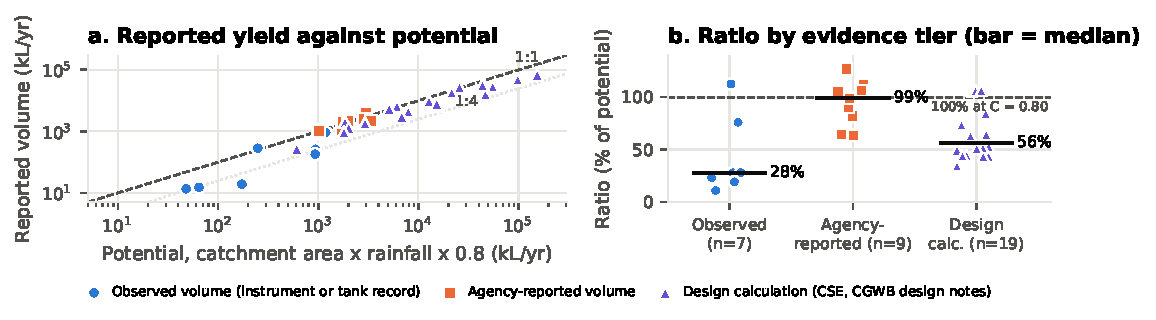
\includegraphics[width=\textwidth]{../figures/fig1_performance_gap.pdf}
\caption{Reported yield against theoretical potential, 35 observations at 31 sites. (a) Reported volume against potential (log scales) with 1:1 and 1:4 lines. (b) Performance ratio by evidence tier (bars are medians). Observed volumes sit well below agency-reported ones, which cluster at 100\% of potential.}
\label{fig1}
\end{figure*}

\begin{figure*}[t]
\centering
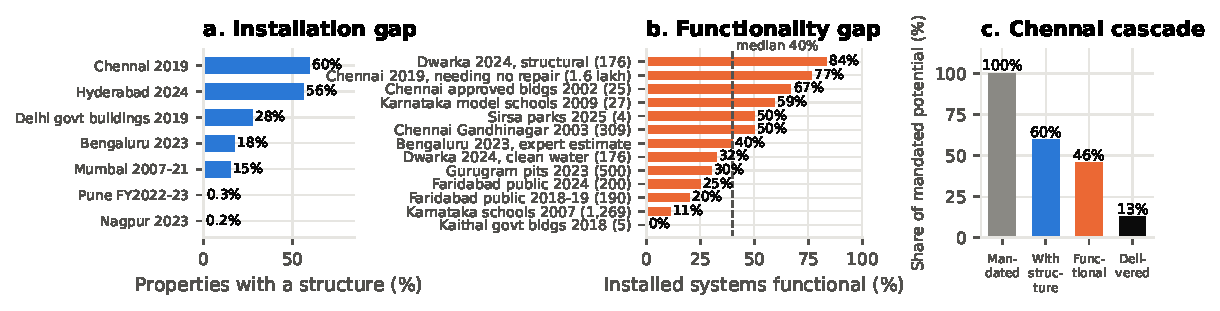
\includegraphics[width=\textwidth]{../figures/fig2_mandate_gap.pdf}
\caption{The mandate gap in three steps. (a) Share of properties with a structure: six city figures and Delhi government buildings. (b) Share of installed systems reported functional, 13 estimates from 12 surveys and audits (sample sizes in brackets). (c) Chennai, one 2019 inspection snapshot: share with a structure, share of those needing no repair, and water delivered at the observed yield ratio.}
\label{fig2}
\end{figure*}

\begin{figure*}[!b]
\centering
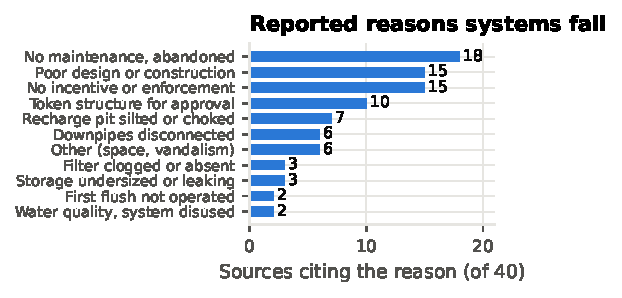
\includegraphics[width=0.425\textwidth]{../figures/fig3_failure_modes.pdf}\hfill
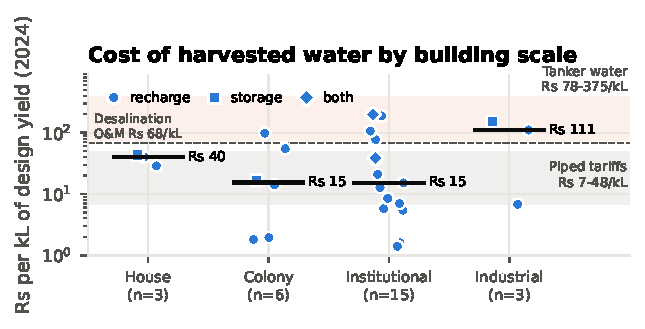
\includegraphics[width=0.56\textwidth]{../figures/fig4_cost_per_kL.pdf}
\caption{Left: reasons for failure, by distinct source among 40 surveys, audits and reports (90 mentions). Right: levelised cost per kL of design yield, 27 systems by building scale (bars are medians; 15-year life, 8\%, O\&M 2\%, 2024 rupees) against piped tariffs, desalination and tanker benchmarks.}
\label{fig34}
\end{figure*}

\textbf{Installation and functionality (Fig.~\ref{fig2}).} Installation shares range from 60\% of 2.72 lakh houses inspected in Chennai (2019) and 56\% in Hyderabad to 18\% of connected properties in Bengaluru and below 1\% in Pune and Nagpur. The 13 functional-share estimates have a median of 40\% (range 0 to 84\%): 77\% of Chennai's 1.62 lakh structures needed no repair, 84\% of 176 Dwarka societies had a working structure but only 32\% recharged water free of faecal coliform [8], and 11\% of 1,269 Karnataka school systems worked in 2007 [9]. Chaining the two Chennai figures from one snapshot with the observed median gives 60\% $\to$ 46\% $\to$ 13\% of mandated potential delivered (12\% with Warud regraded); for Bengaluru about 2\% (its functional share is an expert estimate).

\textbf{Failure modes (Fig.~\ref{fig34}, left).} Of 40 sources, 18 cite no maintenance or abandonment, 15 missing awareness, incentive or enforcement, 15 poor design or construction and 10 token structures built only to obtain an approval. Component faults (silted pits 7, broken conveyance 6, clogged filters 3, first flush 2) are cited less often.

\textbf{Cost per kilolitre (Fig.~\ref{fig34}, right).} For 27 systems the levelised cost at design yield has a median of Rs~21 per kL (IQR 7 to 66, 2024 rupees; Rs~29 at a 15\% discount rate); in this sample recharge systems (Rs~15, n\,=\,22) are cheaper than storage (Rs~43, n\,=\,3). Cost per kL falls steeply with catchment area (Spearman $\rho=-0.74$, $p<0.001$); scale-group differences are not significant at these counts (Kruskal-Wallis $p=0.56$). Twenty rows are CSE Delhi-NCR projects of 2000 to 2004 (median Rs~13); the five post-2010 rows median Rs~98. At observed rather than design yield (multiplier 2.0) the median rises to about Rs~42 per kL, within the range of piped tariffs (Rs~7 to 48) and below desalination O\&M (Rs~68) and tanker water (Rs~78 to 375); the post-2010 systems reach about Rs~200, inside the private-tanker range.

\section{Discussion}
The mandates have increased installation. The evidence does not show that they deliver water: agencies report what they designed (the agency-reported and design tiers have medians of 99\% and 56\% of potential), we found only five metered sites, and those deliver about a quarter of potential. Structures installed is an output indicator; water delivered is the outcome. The failure-mode counts agree: no maintenance is cited most often, missing incentives or enforcement ties with poor design or construction, and the faults listed are ones routine inspection would catch. Two other explanations must be considered. Part of the shortfall is technical: at Ramtek the dug well accepted 19 of 215.7~m$^3$ and the rest overflowed [2], an intake limit, not neglect. And private cost matters for recharge: at observed yield the cost per kL (Rs~42 overall, about Rs~80 for the three houses) is above most domestic piped tariffs (Rs~7 to 48) while the recharge benefit is shared with the neighbourhood, so owners have little reason to maintain a pit; that argues for the incentive recommendation below. Three changes follow: require a flow meter or recharge-well level logger on systems above a size threshold, so performance can be verified at all; tie rebates and penalties to periodic functional inspection, not a one-time completion certificate; and publish installed-versus-functional counts, as Chennai did in 2019.

\textbf{Limitations.} The observed tier is small (seven observations, five sites) with two storage-limited houses and one borderline case, so 28\% is indicative, not representative; publication bias favours showcase systems, which makes the gap estimate conservative. Four observed or agency-reported observations use an IMD city normal and four a CSE city average, not the year's rainfall. Functionality surveys differ in definitions and some reach us only through press reports. Cost rows are dominated by one programme and one city. Associations are not causal. These limits show why metering is needed.

\textbf{Contributions.} Nilay: analysis, report. Vedant: analysis, video presentation. Arjun, Yash: sourcing. AI tools helped with code, figures, searches and drafting (statement in the Supplementary Information).

\section*{References}
\scriptsize\setlength{\parskip}{0pt}
[1] Lok Sabha USQ 2478 (5 Mar 2020) and USQ 1241 (9 Feb 2023), Ministry of Jal Shakti, on MBBL 2016 RWH provisions.
[2] CGWB (2011). \emph{Select Case Studies: Rain Water Harvesting and Artificial Recharge}. New Delhi. cgwb.gov.in/cgwbpnm/download/379.
[3] CSE, RWH case studies and model projects, cseindia.org/rainwater-harvesting-case-studies. [4] CSE (2014). \emph{Urban Rainwater Harvesting: Case Studies}.
[5] Lok Sabha SQ 384 (23 Aug 2004), CGWB impact assessment of rooftop RWH projects, eparlib.sansad.in.
[6] CGWB (2007). \emph{Manual on Artificial Recharge of Ground Water}, Table 7.2, Section 9. cgwb.gov.in/cgwbpnm/download/330.
[7] RBI, \emph{Handbook of Statistics on the Indian Economy}, Table 37.
[8] Delhi Jal Board, action-taken report to the NGT, Dwarka RWH, 2024. [9] Arghyam (2007, 2009), Suvarna Jala school RWH reports.
\end{document}
